% F02_Figura2_Esquema.tex
% Figura 2 del articulo: esquema del metodo en tres etapas (preproceso, cambio de elevacion y
% balance, comparaciones), con los datos y los resultados de cada una.
% Datos a la izquierda (categorias de la Tabla 1), las tres etapas al centro (secciones 3.2, 3.3 y 3.4,
% con las subsecciones 3.2.1 a 3.2.4), resultados a la derecha (secciones 4.1 a 4.3 con su tabla o figura).
% Compilar:  pdflatex F02_Figura2_Esquema.tex
%            pdftoppm -png -r 300 -singlefile F02_Figura2_Esquema.pdf figuras/Figura2_esquema
\documentclass[border=3pt]{standalone}
\usepackage[T1]{fontenc}
\usepackage{mathptmx}
\usepackage[none]{hyphenat}
\usepackage{xcolor}
\usepackage{tikz}
\usetikzlibrary{positioning,arrows.meta,fit,backgrounds,calc}

\definecolor{azul}   {HTML}{1B4F72}
\definecolor{result} {HTML}{B0722A}
\definecolor{neutro} {HTML}{55606B}
\definecolor{verdeok}{HTML}{1F7A6B}
\definecolor{violeta}{HTML}{7B5EA7}

\begin{document}
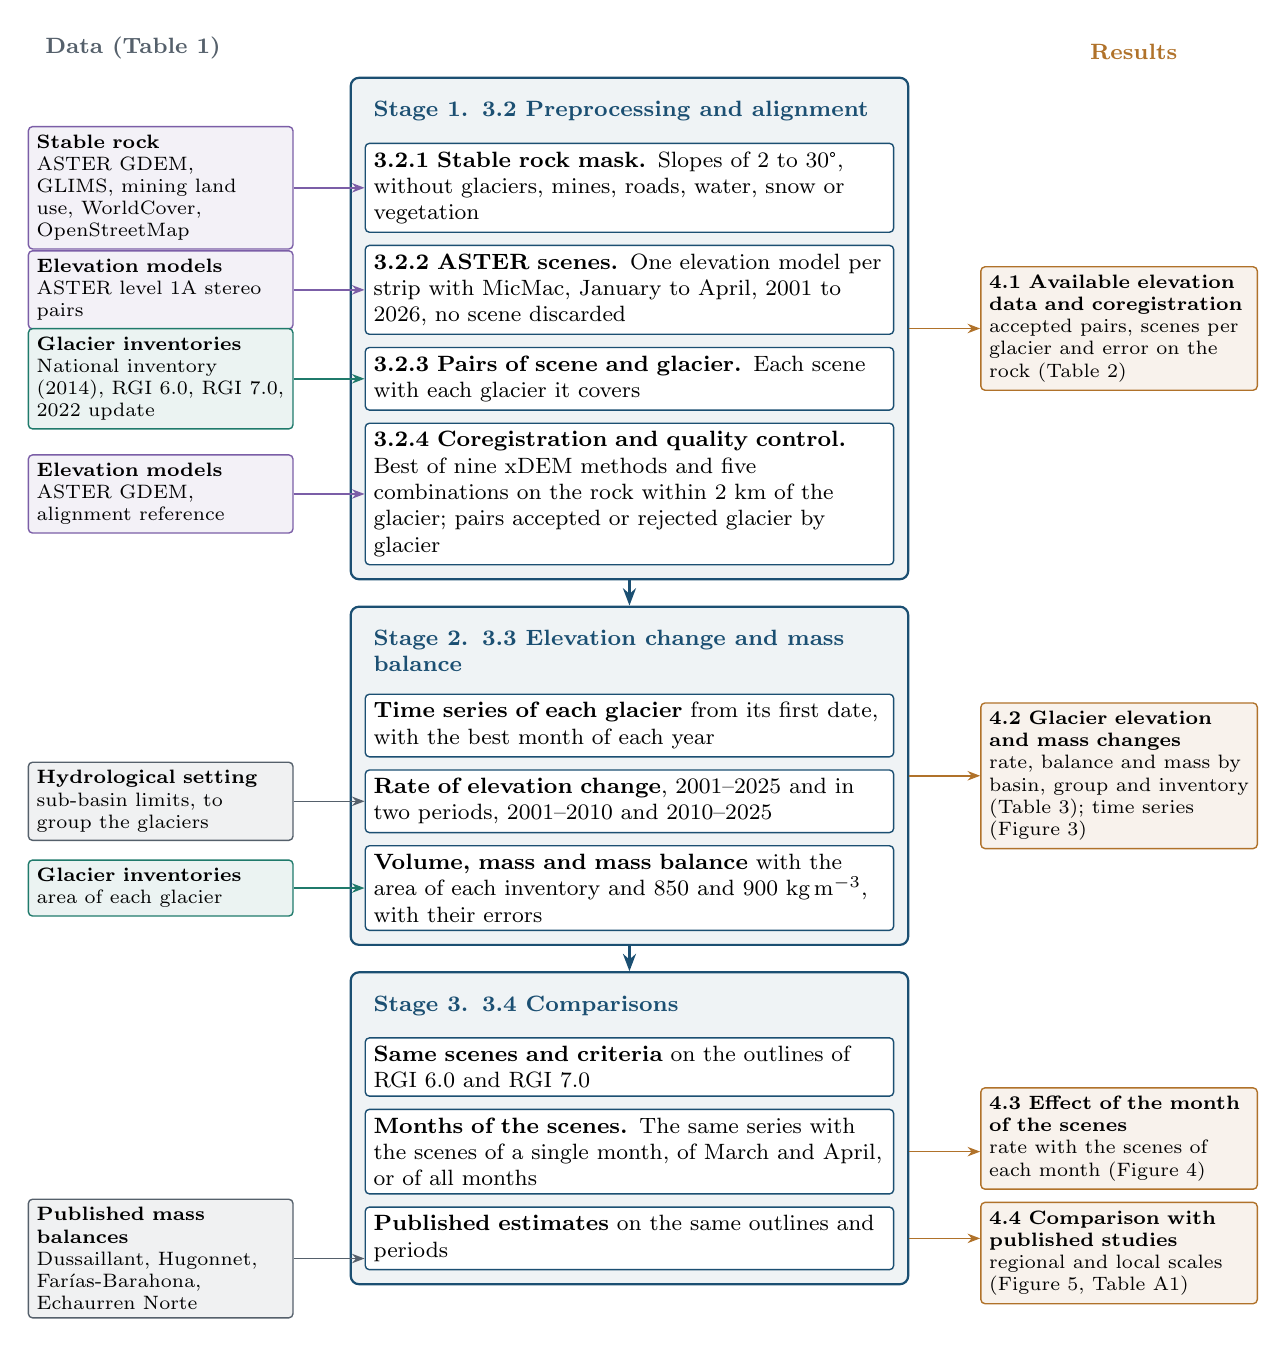
\begin{tikzpicture}[
  font=\footnotesize,
  paso/.style={draw=azul, fill=white, rounded corners=1.5pt, text width=6.5cm, align=left,
               inner sep=3pt, line width=0.5pt},
  etapa/.style={draw=azul, fill=azul!7, rounded corners=3pt, inner sep=5pt, line width=0.8pt},
  titulo/.style={font=\footnotesize\bfseries, text=azul, align=left, text width=6.5cm, inner xsep=3pt},
  dato/.style={draw=#1, fill=#1!9, rounded corners=1.5pt, text width=3.15cm, align=left,
               inner sep=3pt, line width=0.5pt, font=\scriptsize},
  producto/.style={draw=result, fill=result!9, rounded corners=1.5pt, text width=3.3cm,
                   align=left, inner sep=3pt, line width=0.5pt, font=\scriptsize},
  flecha/.style={-{Stealth[length=2.2mm]}, line width=1.1pt, azul},
  aporte/.style={-{Stealth[length=1.6mm]}, line width=0.55pt, #1},
  encab/.style={font=\footnotesize\bfseries, text=#1}
]
% ---------------------------------------------------------------- etapa 1
\node[titulo] (t1) at (0,0) {Stage 1. 3.2 Preprocessing and alignment};
\node[paso, below=1.5mm of t1] (p11) {\textbf{3.2.1 Stable rock mask.} Slopes of 2 to 30\textdegree, without glaciers, mines, roads, water, snow or vegetation};
\node[paso, below=1.5mm of p11] (p12) {\textbf{3.2.2 ASTER scenes.} One elevation model per strip with MicMac, January to April, 2001 to 2026, no scene discarded};
\node[paso, below=1.5mm of p12] (p13) {\textbf{3.2.3 Pairs of scene and glacier.} Each scene with each glacier it covers};
\node[paso, below=1.5mm of p13] (p14) {\textbf{3.2.4 Coregistration and quality control.} Best of nine xDEM methods and five combinations on the rock within 2 km of the glacier; pairs accepted or rejected glacier by glacier};
\begin{scope}[on background layer]
  \node[etapa, fit=(t1)(p11)(p12)(p13)(p14)] (e1) {};
\end{scope}
% ---------------------------------------------------------------- etapa 2
\node[titulo, below=7mm of p14] (t2) {Stage 2. 3.3 Elevation change and mass balance};
\node[paso, below=1.5mm of t2] (p21) {\textbf{Time series of each glacier} from its first date, with the best month of each year};
\node[paso, below=1.5mm of p21] (p22) {\textbf{Rate of elevation change}, 2001--2025 and in two periods, 2001--2010 and 2010--2025};
\node[paso, below=1.5mm of p22] (p23) {\textbf{Volume, mass and mass balance} with the area of each inventory and 850 and 900 kg\,m$^{-3}$, with their errors};
\begin{scope}[on background layer]
  \node[etapa, fit=(t2)(p21)(p22)(p23)] (e2) {};
\end{scope}
% ---------------------------------------------------------------- etapa 3
\node[titulo, below=7mm of p23] (t3) {Stage 3. 3.4 Comparisons};
\node[paso, below=1.5mm of t3] (p31) {\textbf{Same scenes and criteria} on the outlines of RGI~6.0 and RGI~7.0};
\node[paso, below=1.5mm of p31] (p32) {\textbf{Months of the scenes.} The same series with the scenes of a single month, of March and April, or of all months};
\node[paso, below=1.5mm of p32] (p33) {\textbf{Published estimates} on the same outlines and periods};
\begin{scope}[on background layer]
  \node[etapa, fit=(t3)(p31)(p32)(p33)] (e3) {};
\end{scope}
\draw[flecha] (e1.south) -- (e2.north);
\draw[flecha] (e2.south) -- (e3.north);

% ---------------------------------------------------------------- datos (categorias de la Tabla 1)
\node[encab=neutro, anchor=south] at ($(e1.north west)+(-2.75cm,1mm)$) {Data (Table 1)};
\node[dato=violeta, left=9mm of p11] (d1) {\textbf{Stable rock}\\ ASTER GDEM, GLIMS, mining land use, WorldCover, OpenStreetMap};
\node[dato=violeta, left=9mm of p12] (d2) {\textbf{Elevation models}\\ ASTER level 1A stereo pairs};
\node[dato=verdeok, left=9mm of p13] (d3) {\textbf{Glacier inventories}\\ National inventory (2014), RGI~6.0, RGI~7.0, 2022 update};
\node[dato=violeta, left=9mm of p14] (d4) {\textbf{Elevation models}\\ ASTER GDEM, alignment reference};
\node[dato=verdeok, left=9mm of p23] (d5) {\textbf{Glacier inventories}\\ area of each glacier};
\node[dato=neutro, left=9mm of p22] (d6) {\textbf{Hydrological setting}\\ sub-basin limits, to group the glaciers};
% el TanDEM-X salio del texto principal: queda en el apendice con las metodologias anteriores
\node[dato=neutro, left=9mm of p33.north west, anchor=north east, yshift=1mm] (d8) {\textbf{Published mass balances}\\ Dussaillant, Hugonnet, Farías-Barahona, Echaurren Norte};
\draw[aporte=violeta] (d1) -- (p11);
\draw[aporte=violeta] (d2) -- (p12);
\draw[aporte=verdeok] (d3) -- (p13);
\draw[aporte=violeta] (d4) -- (p14);
\draw[aporte=neutro] (d6) -- (p22);
\draw[aporte=verdeok] (d5) -- (p23);
\draw[aporte=neutro] (d8.east) -- (p33.west |- d8.east);

% ---------------------------------------------------------------- resultados
\node[encab=result, anchor=south] at ($(e1.north east)+(2.85cm,1mm)$) {Results};
\node[producto, right=9mm of e1] (r1) {\textbf{4.1 Available elevation data and coregistration}\\ accepted pairs, scenes per glacier and error on the rock (Table 2)};
\node[producto, right=9mm of e2] (r2) {\textbf{4.2 Glacier elevation and mass changes}\\ rate, balance and mass by basin, group and inventory (Table 3); time series (Figure 3)};
\node[producto, anchor=south west] (r3) at ($(e3.east |- p32.south)+(9mm,0.6mm)$) {\textbf{4.3 Effect of the month of the scenes}\\ rate with the scenes of each month (Figure~4)};
\node[producto, anchor=north west] (r4) at ($(e3.east |- p33.north)+(9mm,0.6mm)$) {\textbf{4.4 Comparison with published studies}\\ regional and local scales (Figure~5, Table~A1)};
\draw[aporte=result] (e1.east |- r1) -- (r1);
\draw[aporte=result] (e2.east |- r2) -- (r2);
\draw[aporte=result] (e3.east |- p32) -- (r3.west |- p32);
\draw[aporte=result] (e3.east |- p33) -- (r4.west |- p33);
\end{tikzpicture}
\end{document}
